\chapter{Elaboració d'un PDF tutorial per a principiants}

Ja amb tots els conceptes entesos i la creació de l'app he fet un tutorial per resoldre el cub de Rubik a cegues per a totes les persones que tinguin un domini mínim del cub, és a dir, gent que ja sap fer el cub. 
En comparativa amb el contingut del treball, té algunes semblances, ja que tot està explicat de manera simple i conté algunes coses del treball però també inclou mètodes inicials i altres conceptes que no he introduït al treball perquè a l'hora de fer el cub sense mirar són essencials i, en canvi, a l'hora d'entendre el treball no.\cite{Cuber} \cite{EdgeSetup} \cite{Progressio}
\\\\Si hagués de definir el tutorial amb poques paraules, seria que el contingut està explicat com a mi m'hauria agradat que m'ho haguessin explicat. El resultat del tutorial es pot veure a l'annex 2, encara que no està complet ja que quedaria un annex massa llarg al treball, per veure el tutorial complet he d'anar \href{https://polsances13.github.io/roadto3bld/Tutorial.html}{roadto3bld/tutorial}. Dins de la web hi ha les taules de memorització de les 576 combinacions de dues lletres que es poden fer al 3BLD i és per això que és millor que el tutorial es visualitzi a la web.




\chapter{Elaboració d'una web}

Per deixar-ho tot organitzat he decidit fer una web estàtica\footnote{Una pàgina web estàtica és una pàgina web que es mostra al navegador de l'usuari tal i com està emmagatzemada}. La idea darrere de la web és fer com un tipus de central en la qual et porti als diferents contiguts del treball, en resum està feta perquè serveixi com a tutorial a qualsevol que tingui una mica d'experiència en els cubs i es vulgui inciar en el blind.
Està redactada en HTML5 i CSS3, no és una web molt complexa, però ha sigut desenvolupada sense gairebé experiència prèvia, només aprenent amb tutorials i llibres d'html es pot visitar a \href{https://polsances13.github.io/roadto3bld/index.html}{roadto3bld}.
\\\\Dins de la web hi ha la pàgina principal on hi ha una presentació del contingut de la web, després tenim un menú que porta a les pestanyes de Tutorial, App i Contacte. \cite{AjudaWeb}

\chapter{Piera Open 2023}

Aquest estiu vaig decidir anar a Piera a una competició de cubs de Rubik oficial, regulada per la WCA\footnote{Sigles de World Cube Asociation}. Aquesta competició va ser la meva primera competició oficial, on vaig participar en diferents categories, però prioritzant el 3BLD.
\\\\Les resolucions de 3BLD no van tenir èxit, ja que per aquell moment no tenia confiança i vaig fer DNF a les tres, es pot veure una de les resolucions a \href{https://www.youtube.com/@TDRPolSances}{youtube/tdrpolsances}.
Tot i no tenir èxit, m'emporto l'experiència i fer aquest TdR m'ha motivat més a poder anar a una altra competició i fer una resolució vàlida a 3BLD. Els resultats es poden veure al meu perfil de la WCA (\href{https://www.worldcubeassociation.org/persons/2023GUIR03?event=333bf}{WCA/persons/2023GUIR03}), on es pot comprovar que no tenia prèvies competicions realitzades.

\begin{figure}[!ht]
    \centering
    \rotatebox{-90}{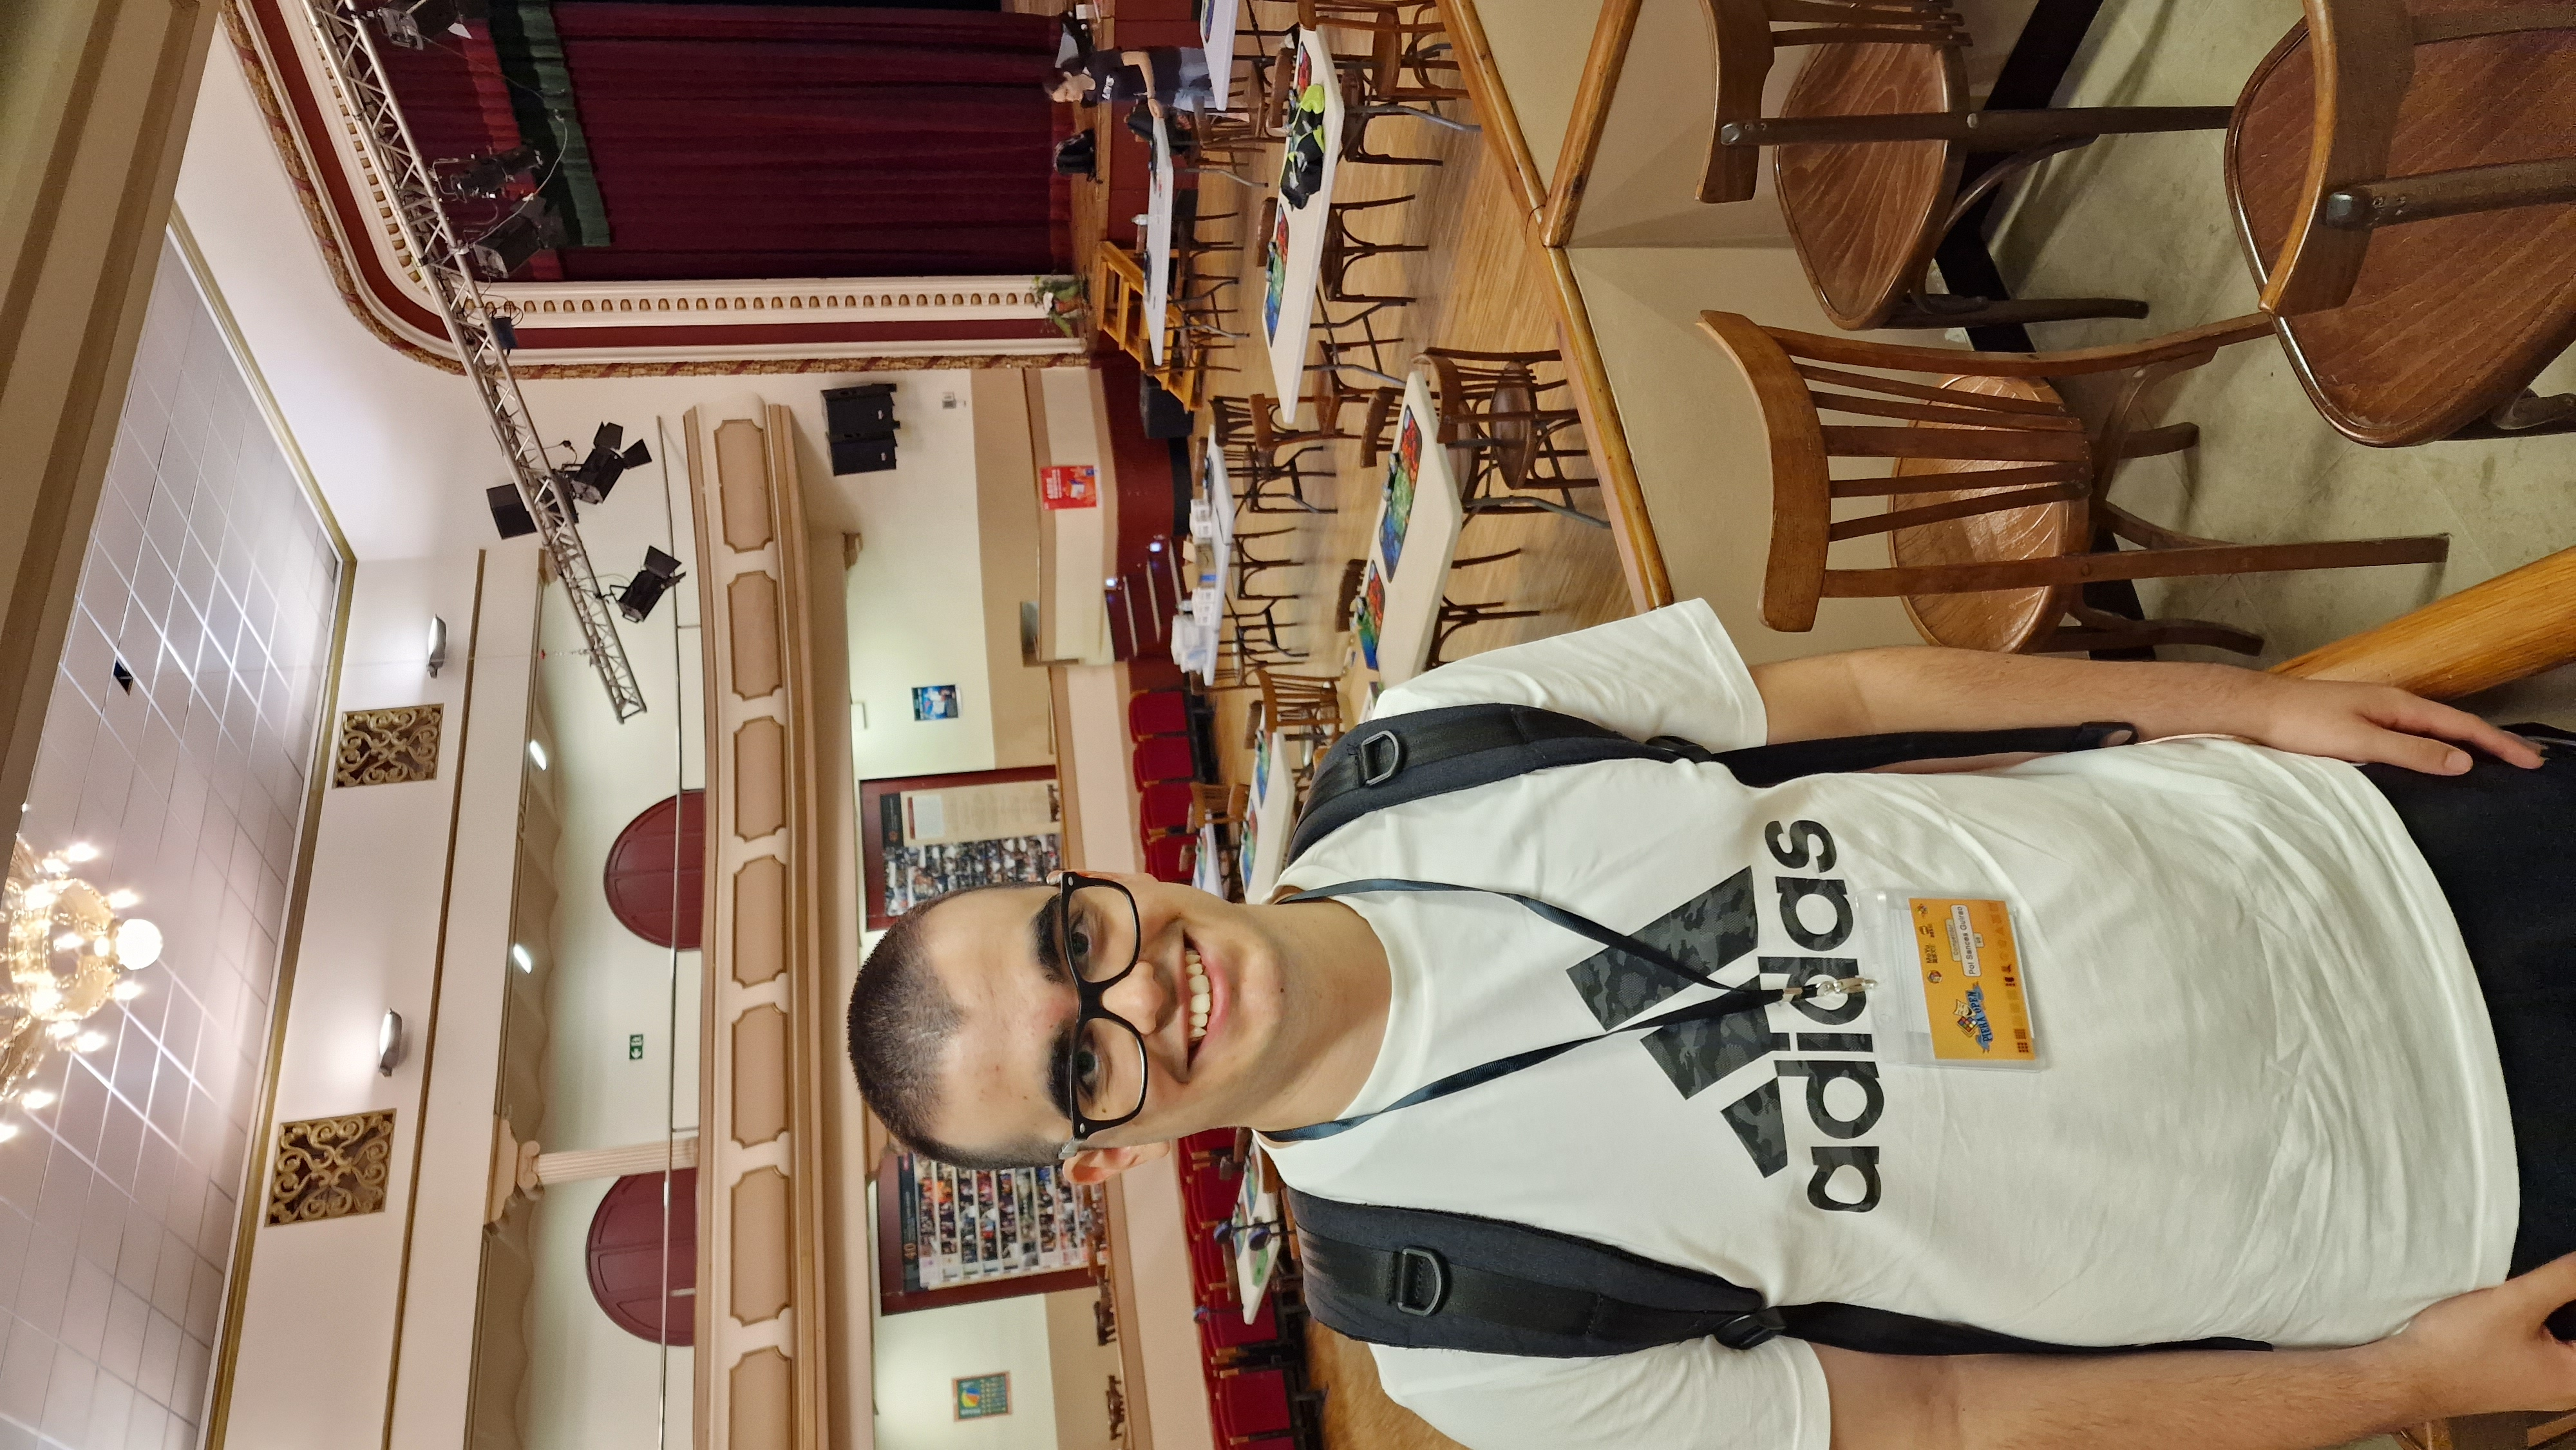
\includegraphics[width=0.4\textwidth]{img/figures/foto-piera.jpg}}
    \caption{Jo al recinte del Piera Open}
    \label{fig:piera}
\end{figure}


\chapter{Resolució del Cub}

Amb tot aquest procés d'aprenentatge he sigut capaç de resoldre el cub de Rubik a cegues. A la competició de Piera encara no estava del tot preparat, però ara que ja he assimilat correctament tots els coneixements he aconseguit resoldre'l en la competició \textit{online} (no-oficial) the cubers.io en 3:40.78 que és un temps bastant raonable. Els resultats de la competició \textit{online}, es poden veure a \href{https://www.cubers.io/u/CUBEANDO_CON_POL/}{cubers.io}.

\begin{figure}[!h]
    \centering
    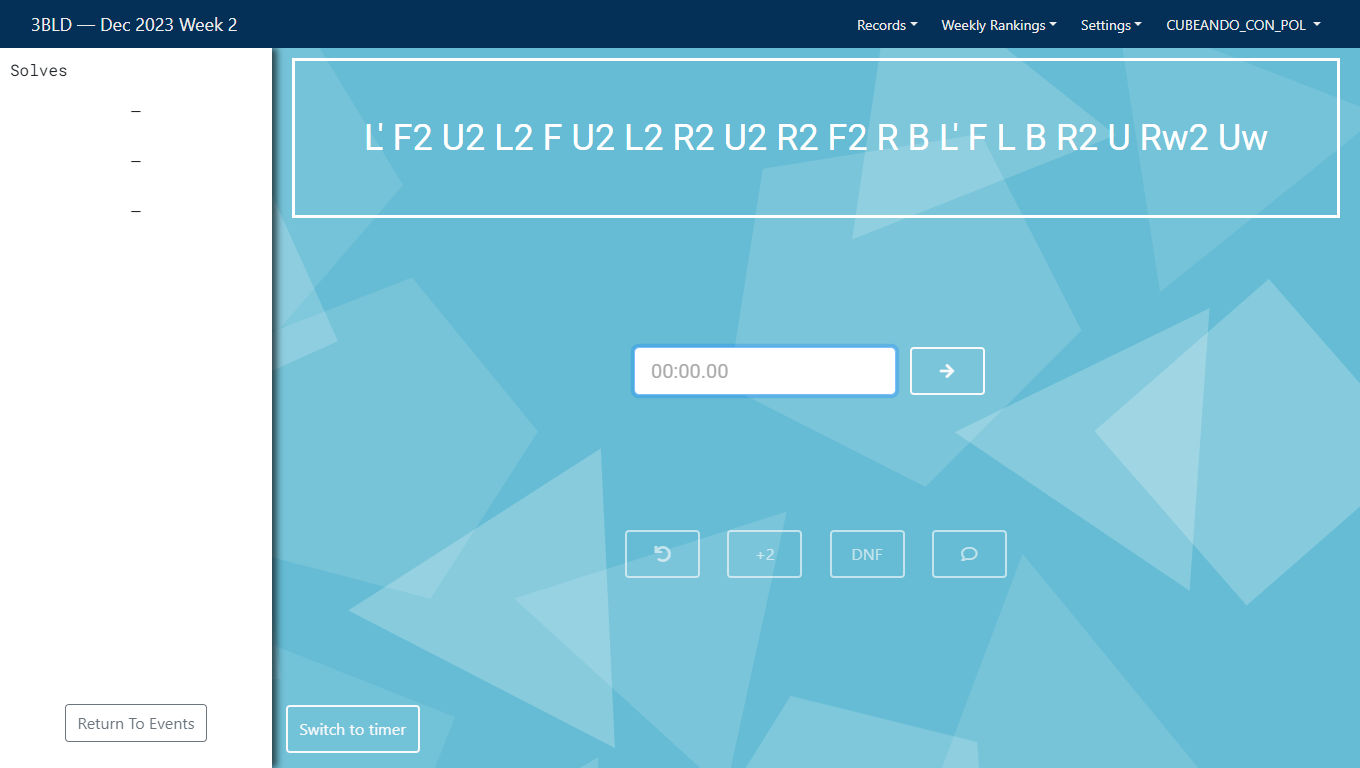
\includegraphics[width=7cm]{img/figures/captura-cubersio.png}
    \caption{Pantalla de barreja de cubers.io}
\end{figure}

Es pot veue un video on faig el cub a cegues a \href{https://www.youtube.com/channel/UCKCx79bCK7JOS4YsgLHbEgA}{youtube.com/TDRPolSances}.
